%Fiquemos com Deus e Nossa Senhora!
%Sao Jose de Cupertino rogai por nos!!
% ### Uses XeLaTeX ### %
% ### Needs beamer-master ### %
\documentclass[aspectratio=169]{beamer} %. Aspect Ratio 16:9

\usetheme{AI2} % beamerthemeSprace.sty
\usepackage[portuguese]{babel}
\usepackage[utf8]{inputenc}
\usepackage[T1]{fontenc}
\usepackage{ragged2e}

% DATA FOR FOOTER
\date{2021}
\title{Regressão Linear}
\author{João Paulo Papa}
\institute{Advanced Institute for Artificial Intelligence (AI2)}

\begin{document}
% ####################################
% FIRST SLIDE 						:: \SliTit{This is the Title of the Talk}{A. B. Name}{Sprace}
% SUB-TITLE SLIDE 					:: \SliSubTit{<title>}{<explanation}
% SUB-SUB-TITLE SLIDE				:: \SliSubSubTit{<title>}{<explanation}
% SLIDE WITH TITLE 					:: \SliT{Title}{Content}
% SLIDE NO TITLE 						:: \Sli{Content} 
% SLIDE DOUBLE COLUMN WITH TITLE 	:: \SliDT{Title}{First Column}{Second Column}
% SLIDE DOUBLE COLUMN NO TITLE 		:: \SliD{First Column}{Second Column}
% SLIDE ADVANCED WITH TITLE 			:: \SliAdvT{Title}{Content}
% SLIDE ADVANCED NO TITLE 			:: \SliAdv{Content}
% SLIDE ADVANCED DOUBLE WITH TITLE 	:: \SliAdvDT{Title}{First Column}{Second Column}
% SLIDE ADVANCED DOUBLE NO TITLE 	:: \SliAdvD{First Column}{Second Column}
% SLIDE BLACK						:: \Black{ <Content> }
% SLIDE WHITE						:: \White{ <Content> }
% ITEMIZATION 						:: \begin{itemize}  \iOn{First} \iTw {Second} \iTh{Third} \end{itemize}
% COMMENT TEXT				 		:: \note{<comment>}
% SECTION 							:: \secx{Section} | \secxx{Sub-Section}
% BOLD SPRACE COLOR				:: \bfs{<text>}
% TABLE OF CONTENT					:: \tocitem{<title>}{<content>}
% LEFT ALIGN EQUATION				:: \begin{flalign*}  & <equation> &   \end{flalign*}
% CENTER ALIGN EQUATION	S			:: \begin{gather*} <equations>  \end{gather*}
% SLASH								:: \slashed{<>}
% BAR								:: \barr{<letter>} instead of \bar{<letter>}
% THEREFORE						:: use \portanto (larger and bold}
% 2 or 3 MATH SYMBOLS				:: \overset{<up>}{<down>} &  \underset{<below>}{\overset{<above>}{<middle>}}  
% INSERT TEXT IN FORMULA			:: \ins{<text>}
% EXERCISE							:: \exe{<exercise #>}{<exercise text>}
% SUGGESTED READING BOX			:: \sug{<references>}
% CITATION							:: \cittex{<citation>}
% CITATION DOUBLE COLUMN 			:: \cittexD{<citation>}
% TEXT POSITION						:: \texpos{<Xcm>}{<Ycm>}{<text>} origin = center of slide : x right | y down
% REFERENCE AT BOTTOM  S/D SLIDE		:: \refbotS{<reference>} \refbotD{<reference>}
% HIDDEN SLIDE						:: \hid
% COLOR BOX 						:: \blu{blue} + \red{rec} + \yel{yellow} + \gre{green} + \bege{beige}
% FRAME 							:: \fra{sprace} \frab{blue} \frar{red} + \fray{yellow} + \frag{green}		
% FIGURE 							:: \img{X}{Y}{<scale>}{Figure.png} 
% FIGURE							:: \includegraphics[scale=<scale>]{Figures/.png}
% FIGURE DOUBLE SLIDE NO TITLE		::  \img{-4}{0.5}{<scale>}{Figure.png} % Image 1st half
%									::  \img{4}{0.5}{<scale>}{Figure.png} % Image 2nd half
% FIGURE DOUBLE SLIDE WITH TITLE		::  \img{-4}{0}{<scale>}{Figure.png} % Image 1st half
%									::  \img{4}{0}{<scale>}{Figure.png} % Image 2nd half
% INCLUDING SWF (Flash)				:: \usepackage{media9} and \includemedia >> USE ACROBAT <<
%%%%%%%%%%%%%%%%%%%%%%%%%%%%%%%%%%%%%%%%%%%%%%%%%%
% ###############################################################################
% FIRST SLIDE
\SliTit{Regressão Linear}{Advanced Institute for Artificial Intelligence -- AI2}{https://advancedinstitute.ai}
%%%%%%%%%%%%%%%%%%%%%%%%%%%%%%%%%%%%%%%%%%%%%%%%%%
% ###############################################################################
% SLIDE SUB-TITLE
%\SliSubTit{Sub-Title}{Description}{}
%%%%%%%%%%%%%%%%%%%%%%%%%%%%%%%%%%%%%%%%%%%%%%%%%%
% ###############################################################################
%\SliSubSubTit{Sub-Sub-Title}{Description}
 %%%%%%%%%%%%%%%%%%%%%%%%%%%%%%%%%%%%%%%%%%%%%%%%%%


\SliT{Introdução}{
\secx{Regressão Linear Univariada}

\justifying Em aprendizado de máquina, existem diversos problemas para os quais conhecemos um conjunto de valores de entrada e desejamos \textbf{estimar} o valor de saída. Um exemplo bastante comum é a precificação de imóveis, cujo valor de entrada corresponde ao tamanho de uma casa e a saída desejada é o seu preço.

\begin{center}
\onslide<2->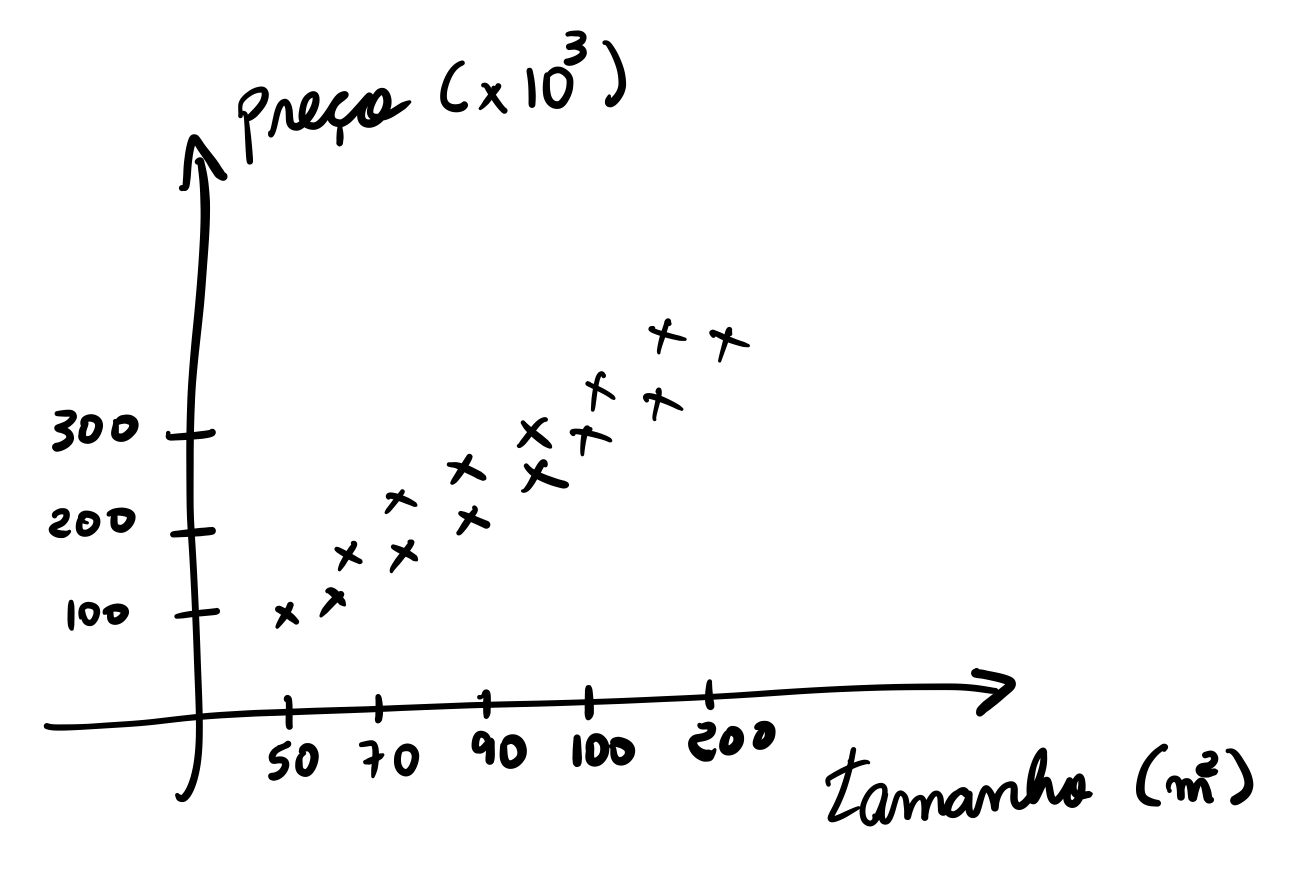
\includegraphics[scale=0.1]{./figs/Regressao_Linear_Fig1.png}
\onslide<3->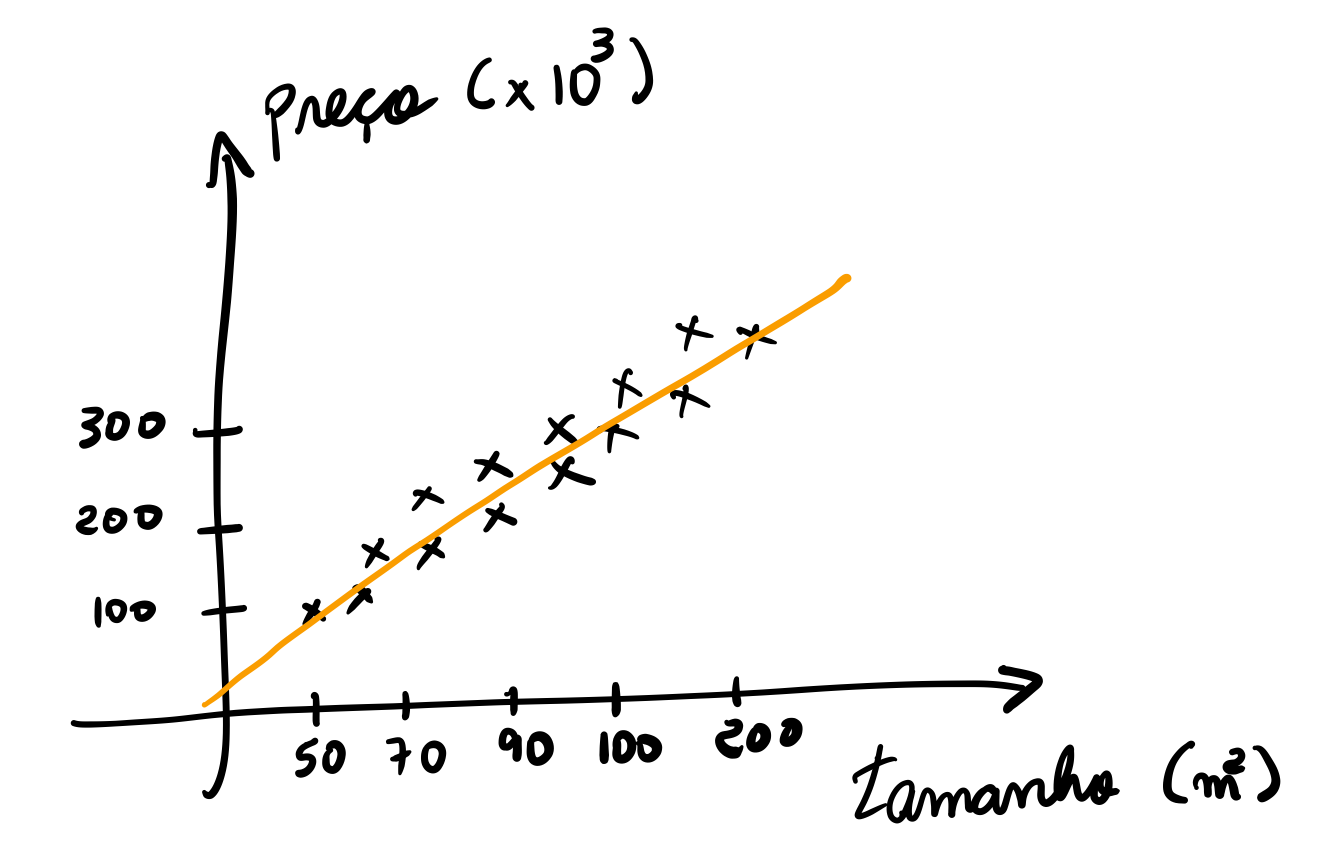
\includegraphics[scale=0.1]{./figs/Regressao_Linear_Fig2.png}
\end{center}

%\secxx{Sub-Section}

% EXERCISE
%\exe{4}{Exercise}
% SUGGESTED READING BOX			
%\sug{References}
% CITATION						
%\cittex{Citation}

}%%%%%%%%%%%%%%%%%%%%%%%%%%%%%%%%%%%%%%%%%%%%%%%%%%
% ###############################################################################
% SLIDE NO TITLE
\Sli{
\underline{Definição do problema:} seja um conjunto de dados ${\cal X}= \{(x_1,y_1),(x_2,y_2),\ldots,(x_m,y_m)\}$ tal que $x_i\in\mathbb{R}$ corresponde ao dado de entrada e $y_i\in\mathbb{R}$ denota o seu respectivo valor de saída. Temos, ainda, que ${\cal X}$ pode ser \textbf{particionado} da seguinte forma: ${\cal X} = {\cal X}^1\cup {\cal X}^2$, em que ${\cal X}^1$ e ${\cal X}^2$ denotam os conjuntos de dados de \textbf{treinamento} e \textbf{teste}, respectivamente. Nosso objetivo é, dado o conjunto de treinamento, aprender uma função $h:\mathbb{R}\rightarrow\mathbb{R}$ que consiga estimar o valor de uma casa dado o seu tamanho.

\begin{center}
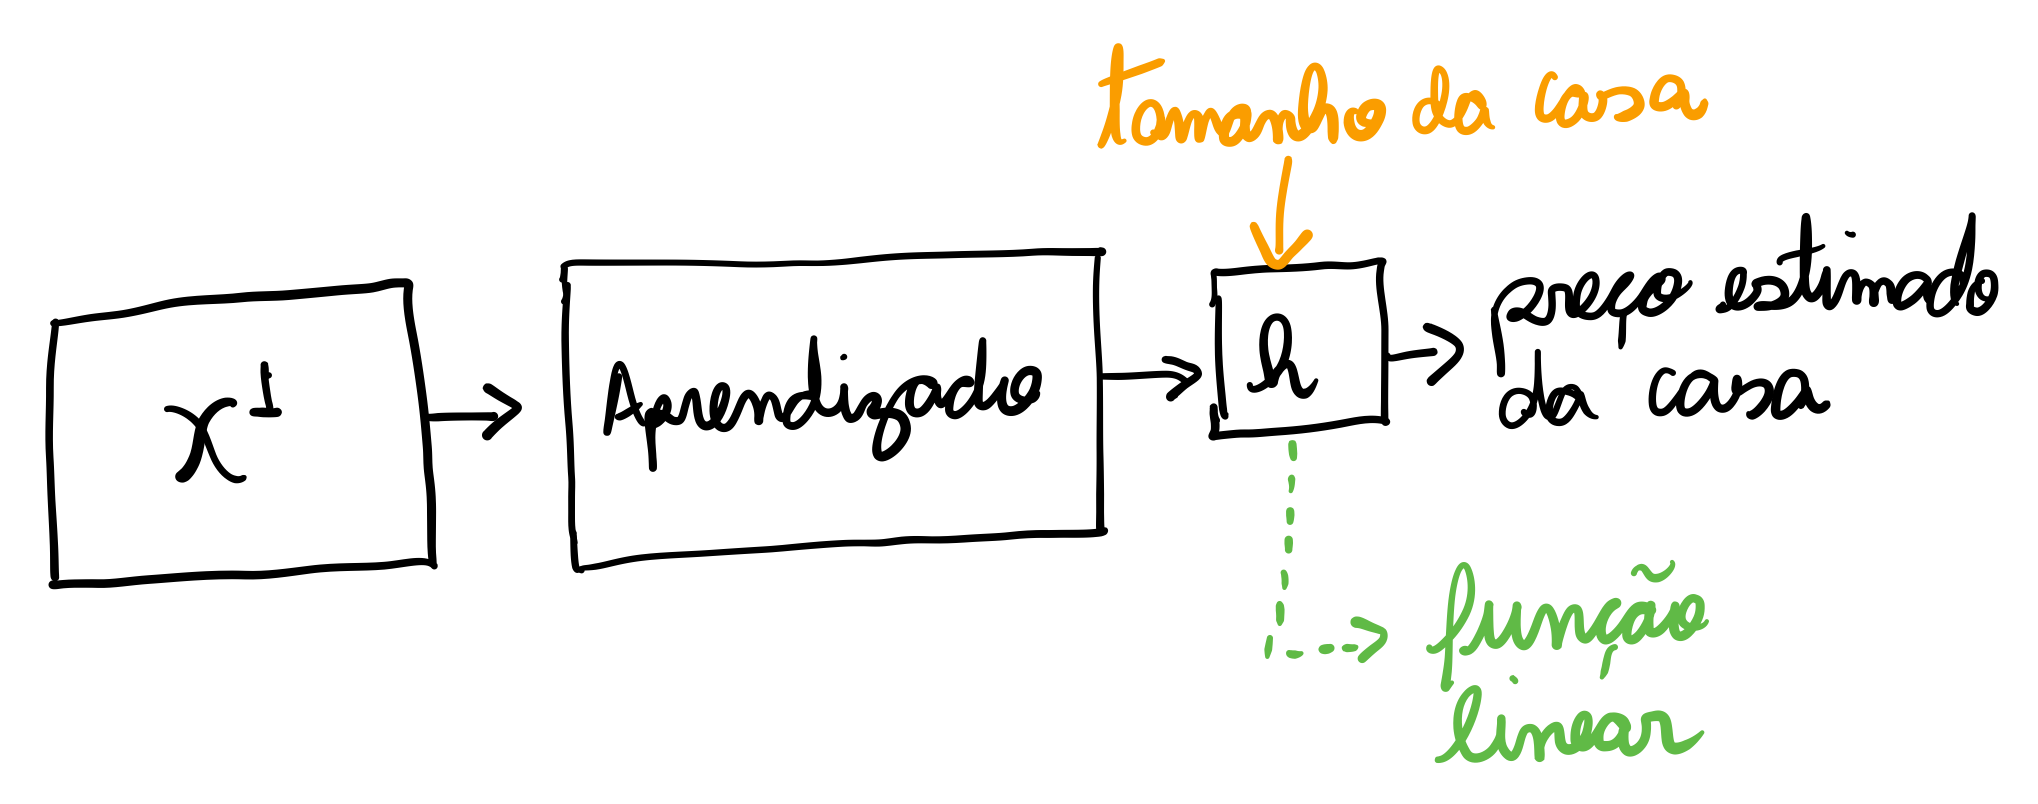
\includegraphics[scale=0.1]{./figs/Regressao_Linear_Fig3.png}
\end{center}

\Sli{

}

}%%%%%%%%%%%%%%%%%%%%%%%%%%%%%%%%%%%%%%%%%%%%%%%%%%
% ###############################################################################
% SLIDE DOUBLE COLUMN WITH TITLE
\SliDT{Title}{First Column}{Second Column

}%%%%%%%%%%%%%%%%%%%%%%%%%%%%%%%%%%%%%%%%%%%%%%%%%%
% ###############################################################################
% SLIDE DOUBLE COLUMN NO TITLE
\SliD{
First Column}{
    { \begin{center}
    
\includegraphics[scale=0.35]{AI2Logo.png}     
    \end{center} }

}%%%%%%%%%%%%%%%%%%%%%%%%%%%%%%%%%%%%%%%%%%%%%%%%%%
% ###############################################################################
% SLIDE ADVANCED  WITH TITLE
\SliAdvT{Advanced Section}{ 
Content

\begin{itemize}
      \iOn{First Level}
   \begin{itemize}
       \iTw {Second Level}
      \begin{itemize}
       \iTh{Third Level}
       \end{itemize}
    \end{itemize}
 \end{itemize}

\refbotS{Reference at the Bottom} 
}%%%%%%%%%%%%%%%%%%%%%%%%%%%%%%%%%%%%%%%%%%%%%%%%%%
% ###############################################################################
% SLIDE ADVANCED  NO TITLE
\SliAdv{ 
Content

\begin{itemize}
      \iOn{First Level}
   \begin{itemize}
       \iTw {Second Level}
      \begin{itemize}
       \iTh{Third Level}
       \end{itemize}
    \end{itemize}
 \end{itemize}

}%%%%%%%%%%%%%%%%%%%%%%%%%%%%%%%%%%%%%%%%%%%%%%%%%%
% ###############################################################################
% SLIDE ADVANCED DOUBLE TITLE 		
\SliAdvDT{Title}{First Column}{Second Column


}%%%%%%%%%%%%%%%%%%%%%%%%%%%%%%%%%%%%%%%%%%%%%%%%%%
% ###############################################################################
% SLIDE ADVANCED DOUBLE NO TITLE 	
\SliAdvD{First Column}{Second Column

}%%%%%%%%%%%%%%%%%%%%%%%%%%%%%%%%%%%%%%%%%%%%%%%%%%
% ###############################################################################
% SLIDE BLACK
\Black{

}%%%%%%%%%%%%%%%%%%%%%%%%%%%%%%%%%%%%%%%%%%%%%%%%%%
% ###############################################################################
% SLIDE WHITE
\White{

}%%%%%%%%%%%%%%%%%%%%%%%%%%%%%%%%%%%%%%%%%%%%%%%%%%
% ###############################################################################
% BOXES & FRAMES
\SliT{Boxes and Frames}{
\[
\yel{\alpha\beta\gamma\delta} + \red{\alpha\beta\gamma\delta} + \gre{\alpha\beta\gamma\delta} + \blu{\alpha\beta\gamma\delta}
\]

\[
\fray{\alpha\beta\gamma\delta} + \frar{\alpha\beta\gamma\delta} + \frag{\alpha\beta\gamma\delta} + \frab{\alpha\beta\gamma\delta}
\]

\[
\fra{\alpha + \beta + \gamma + \delta}
\]

}%%%%%%%%%%%%%%%%%%%%%%%%%%%%%%%%%%%%%%%%%%%%%%%%%%
\SliSubTit{Code Snippets}{Code Snippets Styles}
% FIGURES 
% SLIDE WITH CODE


\begin{SliTC}{Ruby Code - Solarized Light Palette}
  \begin{CodeL}{ruby}
case node[:platform] # node info
when "debian", "ubuntu"
  package "git-core" # package is a resource
else 
  package "git"
end
  \end{CodeL}
\end{SliTC}

\begin{SliTC}{Shell Code - Solarized Dark Palette}
  \begin{CodeD}{bash}
#!/bin/bash
echo "Printing text with newline"
echo -n "Printing text without newline"
echo -e "\nRemoving \t backslash \t characters\n"
  \end{CodeD}
\end{SliTC}

\begin{SliTC}{Python Code - Monokai Palette}
  \begin{CodeM}{python}
# Python Program to calculate the square root
# Note: change this value for a different result
@Teste
num = 8 
# To take the input from the user
num = float(input('Enter a number: '))

num_sqrt = num ** 0.5
print('The square root of %0.3f is %0.3f'%(num ,num_sqrt))
  \end{CodeM}
\end{SliTC}

%%% Slide with black background and code

\begin{BlackC}
  \begin{CodeM}{python}
# Python Program to calculate the square root
# Note: change this value for a different result
@Teste
num = 8 
# To take the input from the user
num = float(input('Enter a number: '))

num_sqrt = num ** 0.5
print('The square root of %0.3f is %0.3f'%(num ,num_sqrt))
  \end{CodeM}
\end{BlackC}


%\begin{BlackC}
%    \begin{CodeD}{python}
%# Python Program to calculate the square root
%# Note: change this value for a different result
%@Teste
%num = 8 
%# To take the input from the user
%num = float(input('Enter a number: '))
%
%num_sqrt = num ** 0.5
%print('The square root of %0.3f is %0.3f'%(num ,num_sqrt))
%    \end{CodeD}
%\end{BlackC}%%%%%%%%%%%%%%%%%%%%%%%%%%%%%%%%%%%%%%%%%%%%%%%%%%%%%%%%%%%%%%%%%5%

% ###############################################################################
\SliSubTit{Figures}{Positioning Figures in the Slide}
% FIGURES 
\Sli{\thispagestyle{empty}
\tikz[remember picture, overlay] \node[anchor=center] at ($(current page.center)+(0,0)$) {(0,0)};
\tikz[remember picture, overlay] \node[anchor=center] at ($(current page.center)+(0,1)$) {(0,1)};
\tikz[remember picture, overlay] \node[anchor=center] at ($(current page.center)+(0,2)$) {(0,2)};
\tikz[remember picture, overlay] \node[anchor=center] at ($(current page.center)+(0,3)$) {(0,3)};
\tikz[remember picture, overlay] \node[anchor=center] at ($(current page.center)+(0,4)$) {(0,4)};
\tikz[remember picture, overlay] \node[anchor=center] at ($(current page.center)+(0,5)$) {(0,5)};
\tikz[remember picture, overlay] \node[anchor=center] at ($(current page.center)+(0,-1)$) {(0,-1)};
\tikz[remember picture, overlay] \node[anchor=center] at ($(current page.center)+(0,-2)$) {(0,-2)};
\tikz[remember picture, overlay] \node[anchor=center] at ($(current page.center)+(0,-3)$) {(0,-3)};
\tikz[remember picture, overlay] \node[anchor=center] at ($(current page.center)+(0,-4)$) {(0,-4)};
\tikz[remember picture, overlay] \node[anchor=center] at ($(current page.center)+(0,-5)$) {(0,-5)};
\tikz[remember picture, overlay] \node[anchor=center] at ($(current page.center)+(1,0)$) {(1,0)};
\tikz[remember picture, overlay] \node[anchor=center] at ($(current page.center)+(2,0)$) {(2,0)};
\tikz[remember picture, overlay] \node[anchor=center] at ($(current page.center)+(3,0)$) {(3,0)};
\tikz[remember picture, overlay] \node[anchor=center] at ($(current page.center)+(4,0)$) {(4,0)};
\tikz[remember picture, overlay] \node[anchor=center] at ($(current page.center)+(5,0)$) {(5,0)};
\tikz[remember picture, overlay] \node[anchor=center] at ($(current page.center)+(6,0)$) {(6,0)};
\tikz[remember picture, overlay] \node[anchor=center] at ($(current page.center)+(7,0)$) {(7,0)};
\tikz[remember picture, overlay] \node[anchor=center] at ($(current page.center)+(8,0)$) {(8,0)};
\tikz[remember picture, overlay] \node[anchor=center] at ($(current page.center)+(-1,0)$) {(-1,0)};
\tikz[remember picture, overlay] \node[anchor=center] at ($(current page.center)+(-2,0)$) {(-2,0)};
\tikz[remember picture, overlay] \node[anchor=center] at ($(current page.center)+(-3,0)$) {(-3,0)};
\tikz[remember picture, overlay] \node[anchor=center] at ($(current page.center)+(-4,0)$) {(-4,0)};
\tikz[remember picture, overlay] \node[anchor=center] at ($(current page.center)+(-5,0)$) {(-5,0)};
\tikz[remember picture, overlay] \node[anchor=center] at ($(current page.center)+(-6,0)$) {(-6,0)};
\tikz[remember picture, overlay] \node[anchor=center] at ($(current page.center)+(-7,0)$) {(-7,0)};
\tikz[remember picture, overlay] \node[anchor=center] at ($(current page.center)+(-8,0)$) {(-8,0)};
\tikz[remember picture, overlay] \node[anchor=center] at ($(current page.center)+(1,1)$) {(1,1)};
\tikz[remember picture, overlay] \node[anchor=center] at ($(current page.center)+(2,2)$) {(2,2)};
\tikz[remember picture, overlay] \node[anchor=center] at ($(current page.center)+(3,3)$) {(3,3)};
\tikz[remember picture, overlay] \node[anchor=center] at ($(current page.center)+(4,4)$) {(4,4)};
\tikz[remember picture, overlay] \node[anchor=center] at ($(current page.center)+(-1,-1)$) {(-1,-1)};
\tikz[remember picture, overlay] \node[anchor=center] at ($(current page.center)+(-2,-2)$) {(-2,-2)};
\tikz[remember picture, overlay] \node[anchor=center] at ($(current page.center)+(-3,-3)$) {(-3,-3)};
\tikz[remember picture, overlay] \node[anchor=center] at ($(current page.center)+(-4,-4)$) {(-4,-4)};
\tikz[remember picture, overlay] \node[anchor=center] at ($(current page.center)+(-1,1)$) {(-1,1)};
\tikz[remember picture, overlay] \node[anchor=center] at ($(current page.center)+(-2,2)$) {(-2,2)};
\tikz[remember picture, overlay] \node[anchor=center] at ($(current page.center)+(-3,3)$) {(-3,3)};
\tikz[remember picture, overlay] \node[anchor=center] at ($(current page.center)+(-4,4)$) {(-4,4)};
\tikz[remember picture, overlay] \node[anchor=center] at ($(current page.center)+(1,-1)$) {(1,-1)};
\tikz[remember picture, overlay] \node[anchor=center] at ($(current page.center)+(2,-2)$) {(2,-2)};
\tikz[remember picture, overlay] \node[anchor=center] at ($(current page.center)+(3,-3)$) {(3,-3)};
\tikz[remember picture, overlay] \node[anchor=center] at ($(current page.center)+(4,-4)$) {(4,-4)};
}%%%%%%%%%%%%%%%%%%%%%%%%%%%%%%%%%%%%%%%%%%%%%%%%%%
% ###############################################################################
\Sli{\thispagestyle{empty}
\tikz[remember picture, overlay] \node[anchor=center] at ($(current page.center)+(0,0)$) {Positions for 4 figures};
\tikz[remember picture, overlay] \node[anchor=center] at ($(current page.center)+(-4,2.25)$) {$\bigotimes$};
\tikz[remember picture, overlay] \node[anchor=center] at ($(current page.center)+(-4,1.5)$) {\footnotesize \bf (-4,2.25)};
\tikz[remember picture, overlay] \node[anchor=center] at ($(current page.center)+(4,2.25)$) {$\bigotimes$};
\tikz[remember picture, overlay] \node[anchor=center] at ($(current page.center)+(4,1.5)$) {\footnotesize \bf (4,2.25)};
\tikz[remember picture, overlay] \node[anchor=center] at ($(current page.center)+(-4,-1.75)$){$\bigotimes$};
\tikz[remember picture, overlay] \node[anchor=center] at ($(current page.center)+(-4,-2.5)$) {\footnotesize \bf (-4,-1.75)};
\tikz[remember picture, overlay] \node[anchor=center] at ($(current page.center)+(4,-1.75)$) {$\bigotimes$};
\tikz[remember picture, overlay] \node[anchor=center] at ($(current page.center)+(4,-2.5)$) {\footnotesize \bf (4,-1.75)};
}%%%%%%%%%%%%%%%%%%%%%%%%%%%%%%%%%%%%%%%%%%%%%%%%%%
% ###############################################################################
\Sli{
\thispagestyle{empty}
% 1 | 2 | 2 | 1 = 6 = 16/6 = 2.67 | 5.33 | 5.33 | 2.67
\tikz[remember picture, overlay] \node[anchor=center] at ($(current page.center)+(0,0)$) {Positions for 3/6 or 8/16 figures};
\tikz[remember picture, overlay] \node[anchor=center] at ($(current page.center)+(0,2.25)$) {$\bigotimes$};
\tikz[remember picture, overlay] \node[anchor=center] at ($(current page.center)+(0,1.5)$) {\footnotesize \bf (0,2.25)};
\tikz[remember picture, overlay] \node[anchor=center] at ($(current page.center)+(-5.33,2.25)$) {$\bigotimes$};
\tikz[remember picture, overlay] \node[anchor=center] at ($(current page.center)+(-5.33,1.5)$) {\footnotesize \bf (-5.33,2.25)};
\tikz[remember picture, overlay] \node[anchor=center] at ($(current page.center)+(5.33,2.25)$) {$\bigotimes$};
\tikz[remember picture, overlay] \node[anchor=center] at ($(current page.center)+(5.33,1.5)$) {\footnotesize \bf (5.33,2.25)};
% 1|2|2|2|1 = 8 : 16/8 = 2 : 2 | 4 | 2 + 2 | 4 | 2 =    -6 -2 2 6
\tikz[remember picture, overlay] \node[anchor=center] at ($(current page.center)+(-6,-1.75)$){$\bigotimes$};
\tikz[remember picture, overlay] \node[anchor=center] at ($(current page.center)+(-6,-2.5)$) {\footnotesize \bf (-6,-1.75)};
\tikz[remember picture, overlay] \node[anchor=center] at ($(current page.center)+(-2,-1.75)$){$\bigotimes$};
\tikz[remember picture, overlay] \node[anchor=center] at ($(current page.center)+(-2,-2.5)$) {\footnotesize \bf (-2,-1.75)};
\tikz[remember picture, overlay] \node[anchor=center] at ($(current page.center)+(2,-1.75)$) {$\bigotimes$};
\tikz[remember picture, overlay] \node[anchor=center] at ($(current page.center)+(2,-2.5)$) {\footnotesize \bf (2,-1.75)};
\tikz[remember picture, overlay] \node[anchor=center] at ($(current page.center)+(6,-1.75)$) {$\bigotimes$};
\tikz[remember picture, overlay] \node[anchor=center] at ($(current page.center)+(6,-2.5)$) {\footnotesize \bf (6,-1.75)};
}%%%%%%%%%%%%%%%%%%%%%%%%%%%%%%%%%%%%%%%%%%%%%%%%%%
% ###############################################################################
\end{document}
